\chapter{Аналитический раздел}

%\par В этом разделе будет проведён анализ предментой области и обзор существующих решений, обоснована актуальность решаемой продуктом задачи. Также, будет формализована задача, пользовательские сценарии, данные и выбрана модель данных, тип базы данных и тип системы управления базой данных. 

\section{Устройство компилятора}

Процесс компиляции состоит из следующих этапов~\cite{compilers}.
\begin{enumerate}
	\item Лексический анализ. 
	\item Синтаксический анализ. 
	\item Семантический анализ.
	\item Генерация кода на языке целевой платформы.
\end{enumerate}

\section{Лексический анализатор}

Лексический анализ~---~распознавание базовых элементов языка, перевод исходной программы в поток лексем и передача токенов, образуемых этими лексемами, последующим стадиям компиляции.


Основные функции лексического анализатора:
\begin{itemize}
	\item удаление пробелов и комментариев, обнаружение лексических ошибок;
	\item сборка последовательности цифр, формирующих константу;
	\item распознавание идентификаторов и ключевых слов.
\end{itemize}

\begin{table}[h!]
	\centering
	\begin{tabular}{p{1\linewidth}}
	  \centering
	  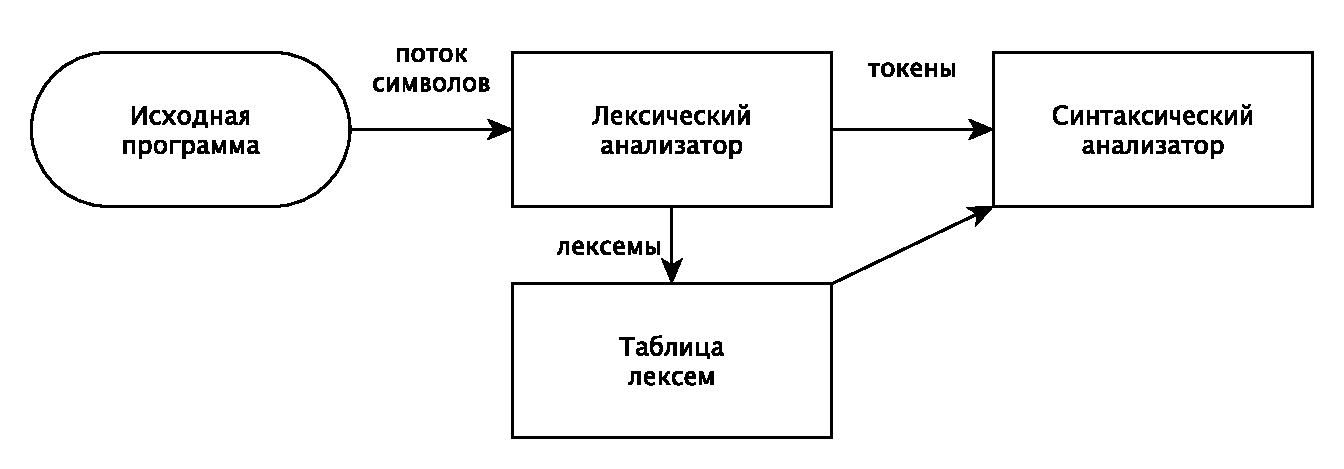
\includegraphics[width=0.8\linewidth]{./images/lexer.pdf}
	  \captionof{figure}{Лексический анализатор}
	  \label{img:lexer}
	\end{tabular}
  \end{table}

\section{Синтаксический анализатор}

Вторая фаза компилятора~---~синтаксический анализ или разбор. Анализатор использует первые компоненты токенов, полученных при лексическом анализе, для создания древовидного промежуточного представления, которое описывает грамматическую структуру потока токенов. 
Типичным представлением является синтаксическое дерево.

Полученная грамматическая структура используется в последующих этапах компиляции для анализа исходной программы и генерации кода для целевой платформы.
Синтаксический анализ выявляет синтаксические ошибки, относящиеся к нарушению структуры программы.

\begin{table}[h!]
	\centering
	\begin{tabular}{p{1\linewidth}}
	  \centering
	  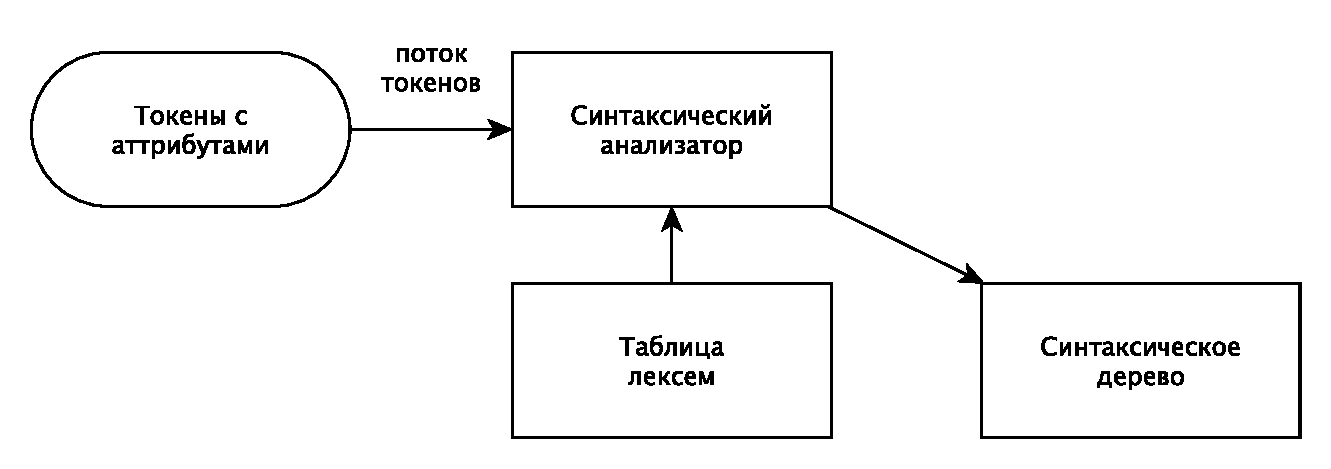
\includegraphics[width=0.8\linewidth]{./images/syntax.pdf}
	  \captionof{figure}{Синтаксический анализатор}
	  \label{img:syntax}
	\end{tabular}
  \end{table}

\section{Семантический анализатор}

Семантический анализатор использует синтаксическое дерево и информацию из таблицы символов для проверки исходной программы на семантическую согласованность с определением языка. Он также собирает информацию о типах и сохраняет все в синтаксическом дереве или в таблице символов для последующего использования в процессе генерации промежуточного кода.

Важной частью семантического анализа является проверка типов, когда компилятор проверяет, имеет ли каждый оператор операнды соответствующего типа.

Как правило, семантический анализатор разделяется на ряд более мелких, каждый из которых предназначен для конкретной конструкции. Соответствующий семантический анализатор вызывается синтаксическим анализатором как только он распознает синтаксическую единицу, требующую обработки.

\begin{table}[h!]
	\centering
	\begin{tabular}{p{1\linewidth}}
	  \centering
	  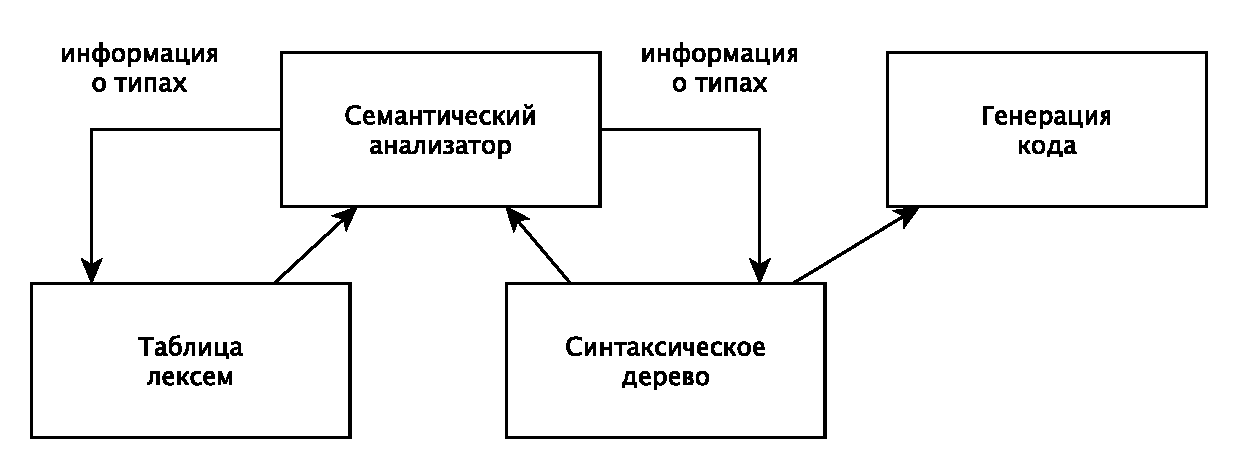
\includegraphics[width=0.8\linewidth]{./images/sem.pdf}
	  \captionof{figure}{Семантический анализатор}
	  \label{img:sem}
	\end{tabular}
  \end{table}

\section{Генерация кода}

\subsection{Генерация промежуточного кода}

В процессе трансляции исходной программы в целевой код компилятор может создавать одно или несколько промежуточных представлений различного вида.
Синтаксические деревья являются видом промежуточного представления. Обычно они используются в процессе синтаксического и семантического анализа.

После синтаксического и семантического анализа исходной программы многие компиляторы генерируют явное низкоуровневое или машинное промежуточное представление исходной программы, которое можно рассматривать как программу для абстрактной вычислительной машины. 
Такое промежуточное представление должно обладать двумя важными свойствами: оно должно легко генерироваться и легко транслироваться в целевой машинный язык.

\subsection{Оптимизация}

Фаза машинно-независимой оптимизации кода пытается улучшить промежуточный код, чтобы затем получить более качественный целевой код. Например, более быстрый код, короткий код, или код, использующий меньшее количество ресурсов. 

\subsection{Генерация кода на целевом языке}

Генератор кода получает в качестве входных данных промежуточное представление исходной программы и отображает его в целевой язык. 
Если целевой язык представляет собой машинный код, для каждой переменной, используемой программой, выбираются соответствующие регистры или ячейки памяти. 
Затем промежуточные команды транслируются в последовательности машинных команд, выполняющих те же действия.

\section{Таблица символов}

Важная функция компилятора состоит в том, чтобы записывать имена переменных в исходной программе и накапливать информацию о разных атрибутах каждого имени. 
Эти атрибуты могут предоставлять информацию о выделенной памяти для данного имени, его типе, области видимости и, в случае имен процедур, такие сведения, как количество и типы их аргументов, метод передачи каждого аргумента, а также возвращаемый тип.
Таблица символов представляет собой структуру данных, содержащую записи для каждого имени переменной, с полями для атрибутов имени. 

\section{Синтаксическое дерево}

Синтаксическое дерево~---~дерево, в котором каждый внутренний узел представляет операцию, а дочерние узлы~---~аргументы этой операции.
Порядок операций в дереве согласуется с обычными правилами, например, умножение имеет более высокий приоритет, чем сложение, и должно быть выполнено до сложения.

\begin{table}[h!]
	\centering
	\begin{tabular}{p{1\linewidth}}
	  \centering
	  \includegraphics[width=1\linewidth]{./images/tree.png}
	  \captionof{figure}{Пример синтаксического дерева}
	  \label{img:tree}
	\end{tabular}
  \end{table}

\section{Генераторы лексических анализаторов}

Существует множество генераторов, наиболее популярные из них~---~Lex, Flex и ANTLR4.

Lex~---~стандартный инструмент для получения лексических анализаторов в операционных системах Unix~\cite{lesk1975lex}. 
В результате обработки входного потока получается исходный файл на языке C. 
Lex-файл разделяется на три блока: блок определений, правил и кода на C. 

Flex заменяет Lex в системах на базе пакетов GNU и имеет аналогичную функциональность~\cite{sampath2007test}.

ANTLR (ANother Tool for Language Recognition)~---~генератор лексических и синтаксических анализаторов, позволяет создавать анализаторы на таких языках, как: Java, C\#, Go, C++ и других~\cite{parr2004s}.

ANTLR генерирует классы нисходящего рекурсивного синтаксического анализатора, на основе правил, заданных грамматикой. 

Он также позволяет строить и обходить деревья синтаксического анализа с использованием паттернов посетитель или слушатель. 
Благодаря своей эффективности и простоте использования, ANTLR является одним из наиболее предпочтительных генераторов анализаторов при создании кода синтаксического анализатора. 
В текущей работе было решено использовать этот инструмент.

\section{Генераторы синтаксических анализаторов}

Для создания синтаксических анализаторов используются такие инструменты, как Yacc/Bison, Coco/R и описанный ранее ANTLR.

Yacc~---~стандартный генератор синтаксических парсеров в Unix системах, Bison~---~аналогичный ему генератор для GNU систем~\cite{yacc}.

Coco/R~---~генератор лексических и синтаксических анализаторов~\cite{mossenbock2003compilergenerator}. 
Лексические анализаторы работают по принципу конечных автоматов, а синтаксические используют рекурсивный спуск. 
Поддерживаются такие языки программирования, как C\+\+, C\#, Java и другие.

Yacc принимает на вход контекстно-свободную грамматику и использует LALR-разбор (LR-разбор с предпросмотром). 
Канонические LR-анализаторы имеют незначительно большую распознавающую способность, чем LALR-анализаторы, однако требуют намного больше памяти для таблиц, поэтому их используют очень редко.

ANTLR и Coco/R принимают на вход контекстно-свободную грамматику, ANTLR использует LL(*)-разбор, а также умеет работать с левой рекурсией, чего не могут
обычные LL-анализаторы, Coco/R использует LL(1)-разбор.

LL-анализатор называется LL(k)-анализатором, если данный анализатор использует предпросмотр на k токенов при разборе входного потока.

LR-анализаторы, в отличие от LL-анализаторов, строящих левосторонний вывод, производят наиболее правую продукцию контекстно-свободной грамматики.
LR-анализ может применяться к большему количеству языков, чем LL-анализ, а также лучше в части сообщения об ошибках, 
то есть он определяет синтаксические ошибки там, где вход не соответствует грамматике, как можно раньше. 
В отличие от этого, LL(k) анализаторы могут задерживать определение ошибки до другой ветки грамматики из-за отката, 
часто затрудняя определение места ошибки в местах общих длинных префиксов. Однако, в большинстве случаев LL-разбор работает быстрее LR-разбора,
а LR-анализаторы и построение их таблиц сложнее в реализации.

\section{LLVM}

LLVM (Low Level Virtual Machine)~---~проект программной инфраструктуры для создания компиляторов и сопутствующих им утилит~\cite{sarda2015llvm}. 
В его основе лежит платформонезависимая система кодирования машинных инструкций~---~байткод LLVM IR. 
LLVM может создавать байткод для множества платформ, включая ARM, x86, x86-64, GPU от AMD и Nvidia и другие. 
Для компиляции LLVM IR в код платформы используется clang. 
В состав LLVM входит также интерпретатор LLVM IR, способный исполнять код без компиляции в код платформы.

LLVM поддерживает целые числа произвольной разрядности, числа с плавающей точкой, массивы, структуры и функции. 
Большинство инструкций в LLVM принимает два аргумента и возвращает одно значение.
Значения в LLVM определяются текстовым идентификатором. 
Тип операндов всегда указывается явно и однозначно определяет тип результата. 
Операнды арифметических инструкций должны иметь одинаковый тип, но сами инструкции «перегружены» для любых числовых типов и векторов.
LLVM IR строго типизирован, поэтому существуют операции приведения типов, которые явно кодируются специальными инструкциями. 
Кроме того, существуют инструкции преобразования между целыми числами и указателями, а также универсальная инструкция для приведения типов bitcast.
Значения в памяти адресуются типизированными указателями. 
Обратиться к ней можно с помощью двух инструкций: load и store. Инструкция alloca выделяет память на стеке. 
Она автоматически освобождается при выходе из функции.
Для вычисления адресов элементов массивов и структур с правильной типизацией используется инструкция getelementptr. 
Она только вычисляет адрес без обращения к памяти, принимает произвольное количество индексов и может разыменовывать структуры любой вложенности.

\section{Вывод}

В данном разделе приведён обзор основных фаз компиляции, описана каждая из них. 
Также был выбран генератор лексического и синтаксического анализаторов~---~ANTLR и LLVM в качестве генератора машинного кода.


















 
